% =============================================================================
% Rozdział 5: Badania eksperymentalne i analiza wyników
% =============================================================================
\chapter{Badania eksperymentalne i analiza wyników}

\section{Założenia redakcyjne rozdziału (anti-generic)}

Przed opracowaniem wyników przyjęto zestaw zasad, które miały zapobiec tworzeniu opisu ogólnego i ,,bezzapachowego'' metodologicznie. Zasady te są jawne i egzekwowane w całym rozdziale:

\begin{enumerate}
  \item \textbf{Tylko dane z repozytorium.} Każda wartość liczbowa pochodzi z plików \texttt{tests/results/test1...test8} oraz z raportów \texttt{raport\_*.txt}. Nie dopisywano danych syntetycznych.
  \item \textbf{Jedna liczba = jeden kontekst.} Przy każdej liczbie podawany jest scenariusz, metryka i warunki (np. próg HPA, profil obciążenia).
  \item \textbf{Brak ,,marketingowego'' języka.} Wnioski są formułowane przez kontrast: co zadziałało, co nie zadziałało i dlaczego.
  \item \textbf{Rozdzielenie obserwacji od interpretacji.} Najpierw prezentowane są fakty (tabele, wykresy), dopiero potem ich interpretacja.
  \item \textbf{Spójność terminologii.} W całym rozdziale użyto tego samego nazewnictwa: \texttt{cpu-cpu}, \texttt{cpu-memory}, \texttt{cpu-custom}, \texttt{io-cpu}, \texttt{io-memory}, \texttt{io-custom}.
\end{enumerate}

\section{Metodyka i zakres danych}

Analiza obejmuje osiem scenariuszy: dwa bazowe bez HPA (\texttt{baseline-cpu}, \texttt{baseline-io}) oraz sześć scenariuszy macierzy badawczej $2\times3$. Dla każdego scenariusza wykorzystano:

\begin{itemize}
  \item raport tekstowy \textit{k6} (RPS, latencje, stopa błędów),
  \item eksporty CSV z Grafany (repliki, CPU per Pod, RAM per Pod, ruch sieciowy Rx),
  \item metadane konfiguracji HPA (CPU 50\%, Memory 70\%, Custom RPS 100/Pod).
\end{itemize}

Wszystkie wykresy w tej wersji pracy zostały wygenerowane ponownie skryptem \texttt{scripts/analyze\_results.py}. Oś czasu została ujednolicona do formatu \textit{minuty od startu testu}, dzięki czemu porównania między scenariuszami nie są zaburzane różnymi godzinami uruchomień.

\section{Wyniki ilościowe}

\subsection{Scenariusze bazowe}

\begin{table}[H]
  \centering
  \begin{tabularx}{\textwidth}{|l|X|X|}
    \hline
    \textbf{Metryka} & \texttt{baseline-cpu} & \texttt{baseline-io} \\
    \hline
    Średni RPS & 66{,}8 & 62{,}4 \\
    p50 & 85{,}3\,ms & 999\,ms \\
    p95 & 2{,}70\,s & 2{,}93\,s \\
    p99 & 567\,ms & 1{,}83\,s \\
    Stopa błędów (\%) & 37{,}70\% & 0{,}17\% \\
    Średnie zużycie CPU (mCPU) & 145 & 58 \\
    Średnie zużycie pamięci (MiB) & 68 & 72 \\
    \hline
  \end{tabularx}
  \caption{Wyniki scenariuszy bazowych (bez HPA)}
  \label{tab:baseline-results}
\end{table}

\textbf{Obserwacja.} Już w punkcie odniesienia widać asymetrię między profilami: \texttt{baseline-cpu} ma wysoki odsetek błędów (37{,}70\%), podczas gdy \texttt{baseline-io} utrzymuje niski błąd, ale wysokie opóźnienie p95 (2{,}93\,s).

\subsection{Scenariusze CPU-bound}

\begin{table}[H]
  \centering
  \begin{tabularx}{\textwidth}{|l|X|X|X|}
    \hline
    \textbf{Metryka} & \texttt{cpu-cpu} & \texttt{cpu-memory} & \texttt{cpu-custom} \\
    \hline
    Średni RPS & 84{,}3 & 67{,}5 & 65{,}4 \\
    p50 & 126\,ms & 86{,}3\,ms & 84{,}2\,ms \\
    p95 & 459\,ms & 2{,}39\,s & 2{,}69\,s \\
    p99 & 349\,ms & 373\,ms & 698\,ms \\
    Stopa błędów (\%) & 0{,}04\% & 38{,}04\% & 37{,}97\% \\
    Amplituda skalowania $A_R$ & 29 & 0 & 1 \\
    Maks. liczba replik & 29 & 1 & 1 \\
    \hline
  \end{tabularx}
  \caption{Wyniki scenariuszy CPU-bound}
  \label{tab:cpu-results}
\end{table}

\textbf{Obserwacja.} Tylko \texttt{cpu-cpu} skaluje się agresywnie (do 29 replik) i radykalnie obniża błędy. Dwie pozostałe strategie zachowują się prawie jak baseline.

\subsection{Scenariusze I/O-bound}

\begin{table}[H]
  \centering
  \begin{tabularx}{\textwidth}{|l|X|X|X|}
    \hline
    \textbf{Metryka} & \texttt{io-cpu} & \texttt{io-memory} & \texttt{io-custom} \\
    \hline
    Średni RPS & 99{,}4 & 62{,}4 & 62{,}4 \\
    p50 & 609\,ms & 998\,ms & 1{,}00\,s \\
    p95 & 700\,ms & 2{,}97\,s & 3{,}01\,s \\
    p99 & 671\,ms & 1{,}83\,s & 1{,}80\,s \\
    Stopa błędów (\%) & 0{,}11\% & 0{,}17\% & 0{,}17\% \\
    Amplituda skalowania $A_R$ & 6 & 0 & 0 \\
    Maks. liczba replik & 7 & 1 & 1 \\
    \hline
  \end{tabularx}
  \caption{Wyniki scenariuszy I/O-bound}
  \label{tab:io-results}
\end{table}

\textbf{Obserwacja.} Także tutaj jedynie \texttt{io-cpu} realnie skaluje usługę i redukuje p95. Strategie Memory i Custom pozostają praktycznie bez reakcji.

\section{Wykresy przebiegu skalowania i zasobów}

\begin{figure}[H]
  \centering
  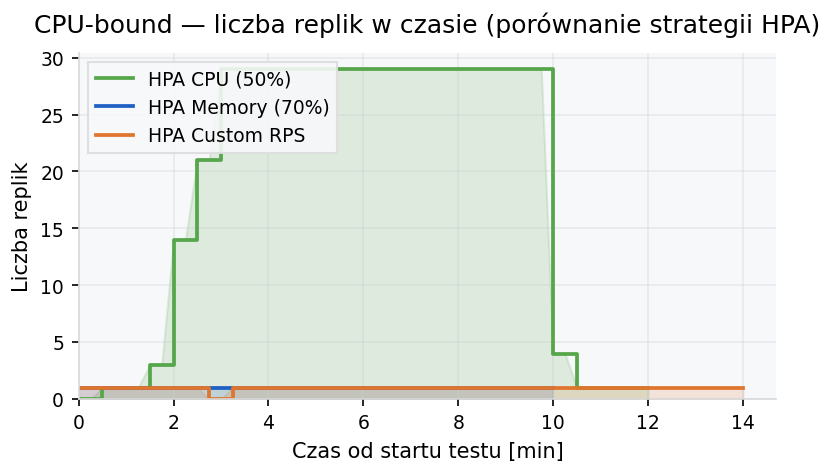
\includegraphics[width=\textwidth]{charts/replicas_cpu_comparison.png}
  \caption{CPU-bound: liczba replik w czasie (oś X: minuty od startu testu)}
  \label{fig:scaling-cpu-comparison}
\end{figure}

\begin{figure}[H]
  \centering
  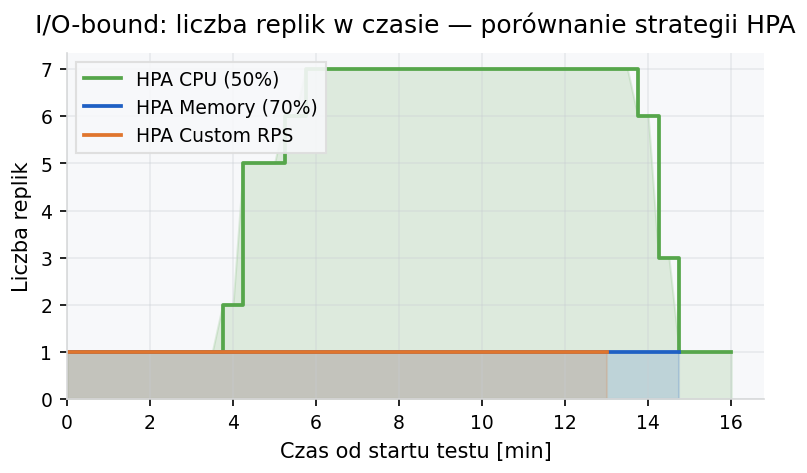
\includegraphics[width=\textwidth]{charts/replicas_io_comparison.png}
  \caption{I/O-bound: liczba replik w czasie (oś X: minuty od startu testu)}
  \label{fig:scaling-io-comparison}
\end{figure}

\begin{figure}[H]
  \centering
  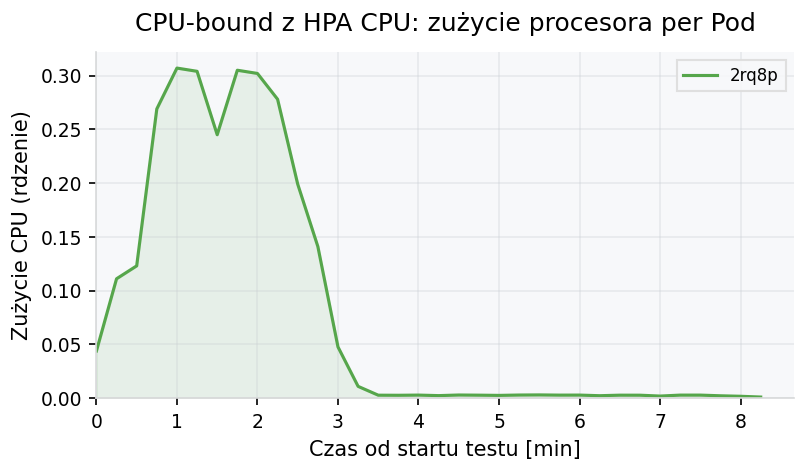
\includegraphics[width=\textwidth]{charts/cpu_usage_cpu_cpu.png}
  \caption{CPU-bound + HPA CPU: zużycie CPU per Pod}
  \label{fig:cpu-usage-cpu-cpu}
\end{figure}

\begin{figure}[H]
  \centering
  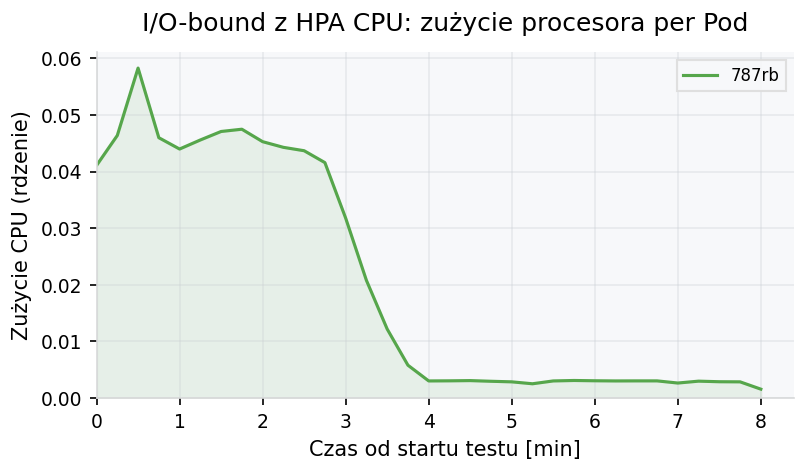
\includegraphics[width=\textwidth]{charts/cpu_usage_io_cpu.png}
  \caption{I/O-bound + HPA CPU: zużycie CPU per Pod}
  \label{fig:cpu-usage-io-cpu}
\end{figure}

\begin{figure}[H]
  \centering
  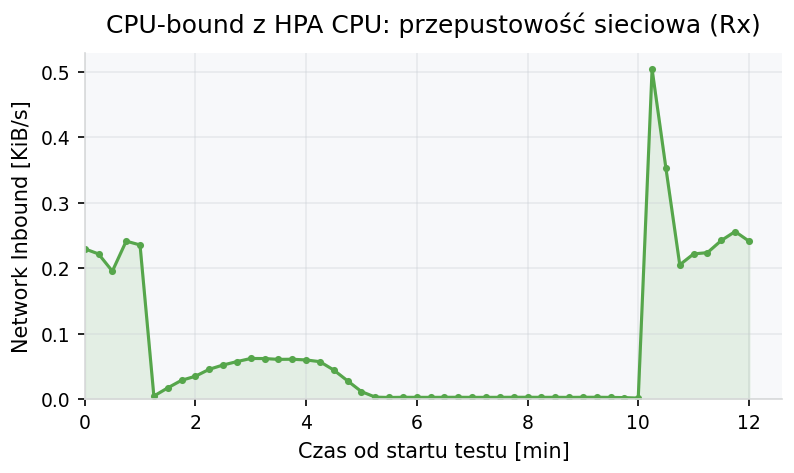
\includegraphics[width=\textwidth]{charts/network_inbound_cpu_cpu.png}
  \caption{CPU-bound + HPA CPU: ruch wejściowy sieci (Rx)}
  \label{fig:network-cpu-cpu}
\end{figure}

\begin{figure}[H]
  \centering
  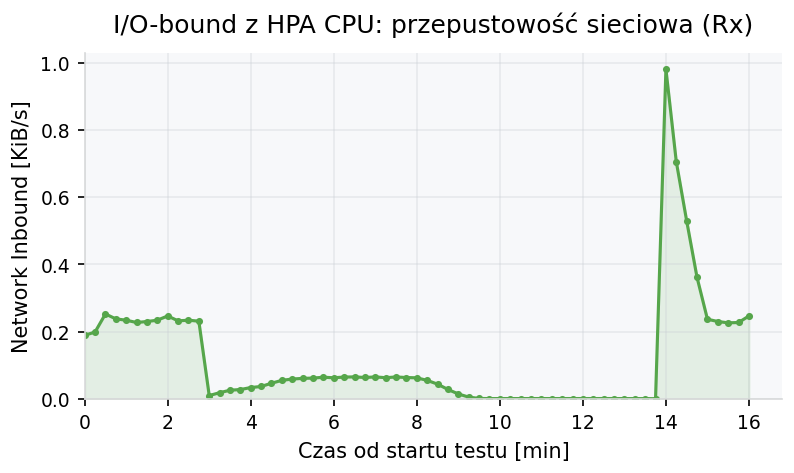
\includegraphics[width=\textwidth]{charts/network_inbound_io_cpu.png}
  \caption{I/O-bound + HPA CPU: ruch wejściowy sieci (Rx)}
  \label{fig:network-io-cpu}
\end{figure}

\begin{figure}[H]
  \centering
  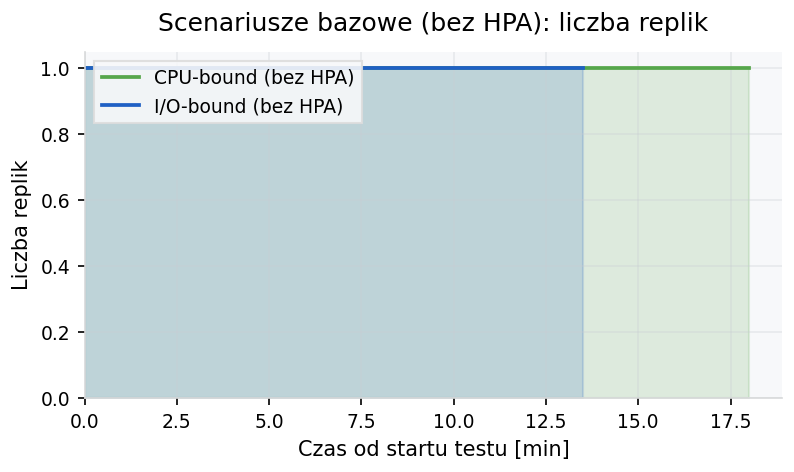
\includegraphics[width=\textwidth]{charts/replicas_baseline.png}
  \caption{Scenariusze bazowe: liczba replik (brak aktywnego HPA)}
  \label{fig:scaling-baseline}
\end{figure}

\section{Interpretacja wyników}

\subsection{Dlaczego HPA CPU działa w obu profilach?}

Wyniki pokazują, że metryka CPU przekroczyła próg zarówno dla \texttt{cpu-service}, jak i \texttt{io-service}. Dla CPU-bound jest to oczekiwane. Dla I/O-bound istotny okazał się narzut współbieżności (obsługa dużej liczby połączeń i przełączeń zadań), który podniósł zużycie CPU na tyle, że HPA zareagował.

\subsection{Dlaczego HPA Memory nie skaluje?}

W obu usługach pamięć ma relatywnie stabilny profil i nie rośnie proporcjonalnie do chwilowego ruchu. Przy progu 70\% nie dochodzi do przekroczenia warunku skalowania, więc liczba replik pozostaje stała.

\subsection{Dlaczego HPA Custom RPS nie skaluje?}

Próg \texttt{100 RPS/Pod} jest za wysoki względem obserwowanego ruchu. Skoro całkowity RPS testu CPU oscyluje w okolicy 65--85, to przy 1--2 replikach metryka per Pod rzadko dochodzi do 100. Wniosek: metryka jest sensowna, ale próg źle skalibrowany dla tych warunków.

\section{Weryfikacja hipotezy i wniosek roboczy}

Hipoteza z Rozdziału 1 jest \textbf{potwierdzona częściowo}. Nie ma jednej metryki działającej dobrze bez strojenia. W badanych warunkach:

\begin{itemize}
  \item HPA CPU jest skuteczny operacyjnie (redukuje błędy i opóźnienia), ale może prowadzić do przeskalowania,
  \item HPA Memory jest nieskuteczny dla badanych usług,
  \item HPA Custom RPS nie zadziałał z powodu kalibracji progu, nie z powodu błędnej idei metryki.
\end{itemize}

Wniosek praktyczny: dobór metryki i strojenie progu muszą być wykonywane razem, na danych z testów obciążeniowych zbliżonych do produkcyjnych.
